\chapter{Optimization Problems}
\label{sec:op}

An optimization problem involves finding the best element among a set of possible alternatives that meet predetermined criteria.
Optimization problems span many domains, including physics, business, and logistics.

\textbf{Rocket.} You have to launch a rocket and land it at a certain point, you have to decide the angle with respect to the ground at which it is launched.

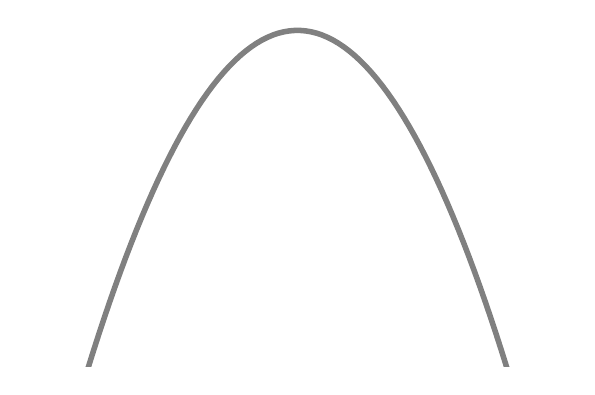
\begin{tikzpicture}
%     \draw[fill=mygreen, mygreen] (0, 0) rectangle (5, 0.25);
    \begin{axis}[
            hide axis,
            ymin=-2, ymax=2,
            xmin=-10, xmax=10
        ]
        \addplot [line width=2pt, domain=-10:10, samples=100, gray] {-1/20*x^2+1};
    \end{axis}
\end{tikzpicture}
\simone{TODO: graph}

\textbf{Travel Salesman's Problem.} Given a list of cities and the distances between each pair of cities, what is the shortest possible route that visits each city exactly once and returns to the starting city?
\simone{TODO: graph}


\textbf{Knapsack.} Given a set of items, each with a weight and a value, determine which items to include in the collection so that the total weight is less than or equal to a given limit and the total value is as large as possible.
\simone{TODO: graph}

\textbf{Position of a Robot.} We have a robot that needs to figure out where it is without a GPS antenna. Antennas have been installed nearby in known locations that can detect the angle between the line connecting the robot to the antenna and the line indicating the direction of the wheels. How can this data be used to calculate the robot's position?
\simone{TODO: graph}

\textbf{Training of Neural Network.} After all, neural networks are complicated optimization problems.
\simone{TODO: graph}

Optimization consists of four steps:
\begin{itemize}
    \item \textbf{Modeling}: in order to work on a problem with a computer, it is necessary to translate the problem into mathematical objects (variables, sets, functions, etc.) that represent it.
    
    \item \textbf{Solving}: Different problems have different characteristics and require analysis to determine the best technique. For example: 
    \begin{itemize}
        \item continuous/discrete: a deliveryman who has to decide how many pizzas to deliver each round must deliver an integer number of pizzas;
        \item linear/nonlinear;
        \item constrained/unconstrained: a car has a maximum speed;
        \item numerical/analytical. 
    \end{itemize}
    After the analysis of the characteristics, it is necessary to find the best algorithm for the solution of the problem.

    \item \textbf{Verification}: every algorithm always return a result (in a certain sense, even a segmentation fault is a result). But is it correct? At this stage, the result is evaluated to see if it makes sense.
    
    \item \textbf{Sensitivity analysis}: the algorithm may be perfect and return the correct result for the desired problem, but the problem may have been inappropriately modeled, e.g. some approximations are inevitable, but if you go too far you will get useless results in reality.
\end{itemize}

There are \underline{no global solutions}, but each problem is unique and requires different modeling, analysis, verification, and sensitivity analysis.


% ---

\section{Modeling}
\label{sec:op.modeling}

Mathematics can represent physical, economic, social, and other phenomenon. These representations in mathematical objects are called \textit{models}, and the process of creating a model is called \textit{modeling}.

A good model must be:
\begin{itemize}
    \item \textbf{accurate enought}: a good model describes phenomena with a high degree of accuracy;
    \item \textbf{sufficiently simple}: a model that is too complex would require more sophisticated algorithms and many computing resources to solve;
    \item \textbf{sufficiently robust/wide}: a good model will be flexible enough to fit a wide range of scenarios.
\end{itemize}

The modeling process involves three steps:
\begin{enumerate}
    \item Identification of \textbf{state variables} (or decision variables): are things that can change in a problem (such as a robot's angle and a rocket's initial velocity). Decisione variables are represented as a column vector \( \mathbb{R}^n \) denoted by \( x \). For example, the variable of a car might be:
    \begin{align*}
        y &= \begin{bmatrix}
                \mathit{angle} \\
                \mathit{velocity} \\
                \mathit{distance} 
             \end{bmatrix}
    \end{align*} 

    \item Identification of a \textbf{ojective function} (or cost/gain function): is the function that evaluates how ``good'' a solution is. Formally it is a function \( f : \mathbb{R}^n \rightarrow \mathbb{R} \). In the car example, an objective function is the distance to the specified destination.
    
    \item Mathemarical description of the \textbf{constraints} (or circumstances): it specifies the constraints that the solution must have. For example, they can be given by physics (e.g. that the velocity must be positive). 
    The set of all solutions satisfying the constraints is called \textbf{feasible set} and is denoted as \( \Omega \).
\end{enumerate}

\begin{outline}
    \textbf{Example.} Consider a box in which we want to maximize the volume by fixing an area.

    \vspace{1em}
   
    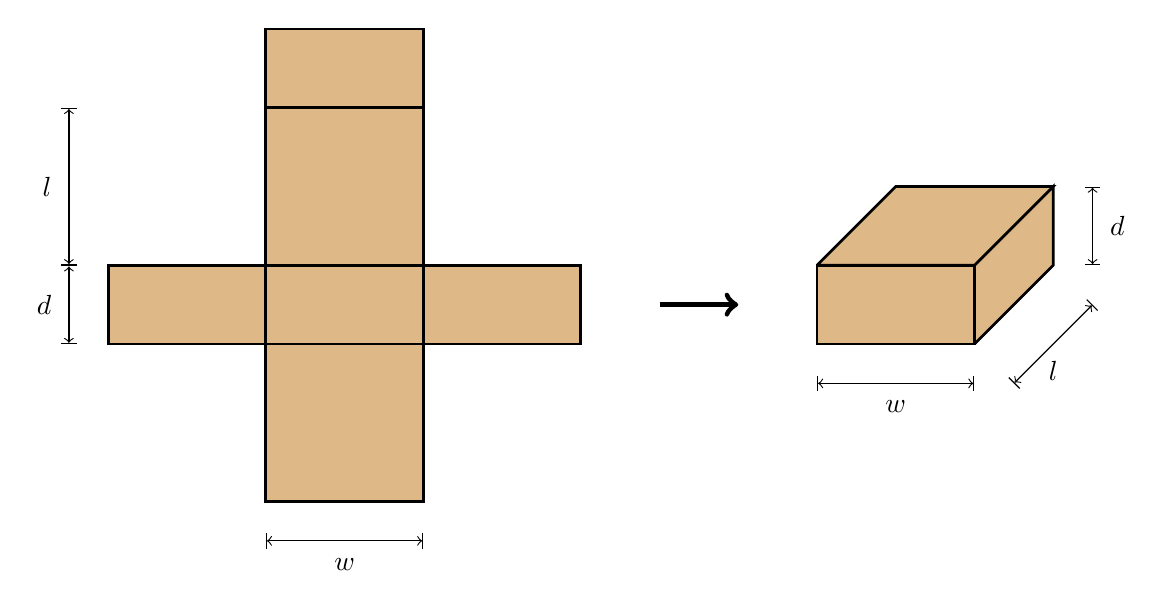
\begin{tikzpicture}
        \definecolor{boxcolor}{RGB}{222,184,135}
        
        % open box
        \draw[fill=boxcolor, line width=1pt] (3,1) rectangle (5,3);
        \draw[fill=boxcolor, line width=1pt] (3,3) rectangle (5,4);
        \draw[fill=boxcolor, line width=1pt] (3,3) rectangle (1,4);
        \draw[fill=boxcolor, line width=1pt] (5,3) rectangle (7,4);
        \draw[fill=boxcolor, line width=1pt] (3,4) rectangle (5,6);
        \draw[fill=boxcolor, line width=1pt] (3,6) rectangle (5,7);

        % quotes of open box
        \draw[|<->|] (0.5, 3) -- node[left=1mm]{\( d \)} (0.5, 4);
        \draw[|<->|] (0.5, 4) -- node[left=1mm]{\( l \)} (0.5, 6);
        \draw[|<->|] (3, 0.5) -- node[below=1mm]{\( w \)} (5, 0.5);

        % arrow
        \draw[->, line width=2px] (8, 3.5) -- (9, 3.5);

        % builded box
        \draw[fill=boxcolor, line width=1pt] (10,3) rectangle (12, 4);
        \draw[fill=boxcolor, line width=1pt] (12,3) -- (13, 4) -- (13, 5) -- (12, 4) -- (12, 3);
        \draw[fill=boxcolor, line width=1px] (10, 4) -- (12, 4) -- (13, 5) -- (11, 5) -- (10, 4);

        % quotes of closed box
        \draw[|<->|] (10, 2.5) -- node[below=1mm]{\( w \)} (12, 2.5);
        \draw[|<->|] (12.5, 2.5) -- node[below=1mm]{\( l \)} (13.5, 3.5);
        \draw[|<->|] (13.5, 4) -- node[right=1mm]{\( d \)} (13.5, 5);
   
    \end{tikzpicture}

    The problem can be modeled as follow:
    \begin{itemize}
        \item \textbf{Decision variables}: \( l, h, w \) in which \( l \) is the length, \( h \) is the height, and \( w \) is the width of the box.
        
        \item \textbf{Constraints}: \( 2lv + 2wh + 2lw = A \) constant. In other words, the area of the box has to be fixed and has to be the same in all the solutions.
        
        \item \textbf{Objective function}: \( V(l, h, w) = l \cdot h \cdot v \). Note: the goal is \( \underset{l, h, w}{\mathit{max}}~V(l, h, w) \).
    \end{itemize}

\end{outline}


% --

\section{Constraints}
\label{sec:op.contraints}

As anticipated in \Cref{sec:op.modeling}, not all possible solutions are good. Depending on the actual problem we are solving, there may be limitations, for example:
\begin{itemize}
    \item we need to calculate the optimal speed of a train, but we cannot choose a negative speed;
    \item to allocate a portfolio, we have to decide the percentage of stocks and bonds based on different parameters, the sum of bonds and stocks must be 100\%;
    \item we have to find the best arrangement of packages in a van. The total weight must not exceed the permitted weight of the vehicle.
\end{itemize}

Constraints take the form of real-valued functions in two possible forms, let \( x \in \mathbb{R}^2 \) a solution, the contraints types are:
\begin{align*}
    h(x) = 0 && \mathrm{equality~constraints} \\
    g(x) \leq 0  && \mathrm{inequality~constraints}
\end{align*}

Formally, given a set of functions (called \textit{equality constraints}) \( \{ h_i(x) \}_m \) where \( m \) is the number of equality constraints, and a set of functions (called \textit{inequality contraints}) \( \{ g_j \}_j \) where \( j \) is the number of inequality contraints, then the \textit{feasible set} \( \Omega \subseteq \mathbb{R}^n \) is
\[ 
    \Omega = \left\{ 
        x \in \mathbb{R}^n   
        \middle\vert
        \begin{array}{l}
            h_i(x) = 0, \quad i = 1, ..., m \\
            g_j(x) \leq 0, \quad j = 1, ..., p
        \end{array}
    \right\}
\]

Taking the above examples again, the train speed is \( x \) and the contraint is \( g_1(x) = -x \). In the wallet example, \( x_1 \) reperesents the percentage of the bonds and \( x_2 \) reperesents the percentage of the stocks, the contraint is \( h_1(x_1, x_2) = x_1 + x_2 - 100 \). Finally, considering the packages in the van \( x_1, ..., x_n \) are the weight of the \( n \) packages, and the constant \( w \) is the maximum weight, the contraint is \( g_1(x1, ..., x_n) = x_1 + x_2 + ... + x_n - w = \sum\limits_{i = 1}^{n} x_n - w \).

\paragraph{Circle.} The choosen solution must be a point in the circumnference of radius \( 1 \). 

\begin{minipage}{0.48\linewidth}
    \center
    \begin{equation*}
        \begin{split}
            \mathit{radius} = 1         & \Rightarrow \\
            \mathit{radius} - 1 = 0     & \Rightarrow \\
            h_1(x, y) = x^2 + y^2 - 1     &
        \end{split}
    \end{equation*}
\end{minipage}
\begin{minipage}{0.5\linewidth}
    \center
    \begin{tikzpicture}
        % \draw (0,0) rectangle (6,6); %create a bounding box to reserve space
        \begin{axis}[
                axis lines=middle, 
                height=5cm,
                width=5cm,
                ymax=1.5, ymin = -1.5,
                xmax=1.5, xmin = -1.5
            ]
            \draw[line width=1pt, myred] (axis cs: 0, 0) circle [radius=1];


        \end{axis}
    \end{tikzpicture}
\end{minipage}

\paragraph{First quadrant.} We want to limit the solutions to be in the first quadrant. In order to do that, we introduce the following condition:

\begin{minipage}{0.49\linewidth}
    \center
    \( 
        x \geq 0 \land y \geq 0 =>  
        \left\{
        \begin{array}{l}
            g_1(x, y) = -x \\
            g_2(x, y) = -y
        \end{array}\right.
    \)
\end{minipage}
\begin{minipage}{0.49\linewidth}
    \center
    \begin{tikzpicture}
        \begin{axis}[
                axis lines=middle,
                height=5cm,
                width=5cm,
                ticks=none,
                ymax=3, ymin=-3,
                xmax=3, xmin=-3
            ]
            \fill[myred!30] (0,0) rectangle (3,3);
        \end{axis}
    \end{tikzpicture}
\end{minipage}

\paragraph{Colors.} \( n \) primary colors are used, which are mixed to form the color required by the client. Of each color \( x_i \), the operator must choose how much to put in and the sum must be exactly the liters requested by the user. To formalize that the sum of the quantities of each color must be exactly \( S \), the constraint is:
\[ h_1(x_1, ..., x_n) = x_1 + x_2 + ... + n_x - S \]


% ---

\section{Minimization}
\label{sec:op.minimization}

To solve an optimization problem, it is necessary to introduce the concept of an objective function (see \Cref{sec:op.modeling}), which, given a solution, gives us a value that indicates how ``good'' it is. If we could find the solution where the function is maximum (or minimum, as the case may be), we would have solved the problem. 

In the end, solving an optimization problem is nothing more than finding the minimum of a function in n variables, where n is the number of parameters that can vary (state variables).
Conventionally in optimization problems we focus on finding the minimum, if the best solution is found at the maximum, we simply invert the function and still find the minimum.

\begin{remark}{black}{white}
    \begin{definition}[minimization problem]
        Find the \( x \in \Omega \) that minimize \( f \).
    \end{definition}
\end{remark}

\begin{remark}{black}{white}
    \begin{definition}[local minimum]
        A point \( x^* \in \Omega \) is a local minimum (or relative minimum) for \( f \) in \( \Omega \) if \( \exists \epsilon > 0 \) such that
        \[
            f(x^*) \leq f(x) \qquad \forall x \in \Omega \mathrm{~such~that~} \mathit{dist}(x, x^*) \leq \epsilon
        \]
    \end{definition}
\end{remark}

In other words, it is a point where the function has a lower value than all other nearby points.

\begin{center}
    \begin{tikzpicture}[scale=0.95]
        \filldraw[black] (5,0) circle (2pt) node[anchor=north]{local min};
        \draw (0,0) to[out=90,in=180] (2,2) to[out=0,in=180] (5,0) to[out=0,in=180] (7,3);
    \end{tikzpicture}
\end{center}

\begin{remark}{black}{white}
    \begin{definition}[strict local minimum]
        A point \( x^* \in \Omega \) is a strict local minimum for \( f \) in \( \Omega \) if \( \exists \epsilon > 0 \) such that
        \[
            f(x^*) < f(x) \qquad \forall x \in \Omega \mathrm{~such~that~} x^* \neq x \land \mathit{dist}(x, x^*) \leq \epsilon
        \]
    \end{definition}
\end{remark}

That is, the function has a higher (not equal) value at nearby points. In other words, "plateaus" are not allowed.

\begin{tikzpicture}[scale=0.95]
    \draw (0,0) to[out=90,in=180] (2,2) to[out=0,in=180] (5,0) to[out=0,in=180] (7,3);
    \filldraw[black] (5,0) circle (2pt) node[anchor=north]{strict local min};

    \draw (10,0) to[out=90,in=180] (12,2) to[out=0,in=180] (14,1.5) to[out=0,in=180] (15.5,1.5) to[out=0,in=-110] (16.5,2.5);
    \filldraw[black] (14.75,1.5) circle (2pt) node[anchor=north]{(non strict) local min};
\end{tikzpicture}

\begin{remark}{black}{white}
    \begin{definition}[global minimum]
        A point \( x^* \in \Omega \) is a global minimum for \( f \) in \( \Omega \) if
        \[
            f(x^*) \leq f(x) \qquad \forall x \in \Omega
        \]
    \end{definition}
\end{remark}

In other words, the smallest local minimum.

\begin{center}
    \begin{tikzpicture}[scale=0.95]
        % \draw (0,1) to[out=-40,in=180] (3,2) to[out=0,in=180] (5,0) to[out=0,in=180] (7,3) to[out=0, in=190] (10, 2) to[out=10, in=-110] (11, 3);
    
        \draw 
            (0,2) to[out=-40, in=180] 
            (1,1) to[out=0, in=190] 
            (3,2) to[out=10, in=180]
            (5,0) to[out=0, in=210]
            (7, 2.5) to[out=20, in=180]
            (9,2) to[out=0, in=230]
            (10, 3)
            ;
    
        \filldraw[black] (5, 0) circle (2pt) node[anchor=north]{global min};
        \filldraw[black] (1, 1) circle (2pt) node[anchor=north]{local min};
        \filldraw[black] (9, 2) circle (2pt) node[anchor=north]{local min};
    \end{tikzpicture}
\end{center}

In the case of a global minimum, we write \( f(x^*) = \underset{\Omega}{\mathtt{min}}f \) and \( x^* = \underset{\Omega}{\mathtt{argmin}} f \). 

Proceed in a similar manner to create the maximum (\( \mathtt{max} \)).

\begin{remark}{gray}{white}
    Note: The words \textit{minimum} and \textit{maximum} refer to the coordinates of the point, not the value of the function.

    % \begin{center}
    %     \begin{tikzpicture}
    %         \begin{axis}[
    %             axis lines=middle
    %           ]
    %           \addplot [line width=1pt, domain=-8:0, samples=100, myred] {(2^x-1)};
    %           \addplot [line width=1pt, domain=0:8, samples=100, myred] {()};
    %         \end{axis} −
    %     \end{tikzpicture}    
    % \end{center}
\end{remark}

\begin{remark}{black}{white}
    \begin{definition}[infimum]
        The infinum of a function \( f : \Omega \rightarrow \mathbb{R} \) is the \textbf{value} \( \mathcal{M} \) such that:
        \begin{itemize}
            \item \( f(x) \geq \mathcal{M} \) for every \( x \in \Omega \);
            \item there is no \( \mathcal{M}' > \mathcal{M} \) such that \( f(x) \geq \mathcal{M}' \) for every \( x \in \Omega \). 
        \end{itemize}
    \end{definition}
\end{remark}

Every function has a infinum! It is not always a minimum. In fact, some functions have no minimum.

\begin{minipage}{0.5\textwidth}
    \begin{tikzpicture}
        \begin{axis}[axis lines=middle, 
                     ticks=none,
                     ymin=-3]
            \addplot [line width=1pt, dashed, domain=-5:3, samples=100, gray] {-1};
            \addplot [line width=1pt, domain=-5:3, samples=100, myred] {2^x-1};
        \end{axis}
    \end{tikzpicture}
    \begin{center}
        \( \mathtt{inf} f = -1 \)

        \( \nexists x \) such that \( f(x) = -1 \), then \( \nexists \mathtt{min} f \)
    \end{center}
\end{minipage}
\begin{minipage}{0.5\textwidth}
    \begin{tikzpicture}
        \begin{axis}[axis lines=middle, 
                     ticks=none,
                     ymax=30]
            \addplot [line width=1pt, domain=-4:2, samples=100, myred] {-x^2+10};
        \end{axis}
    \end{tikzpicture}

    \begin{center}
        \( \mathtt{inf} f = -\infty \)

        \( \nexists x \) such that \( f(x) = -\infty \), then \( \nexists \mathtt{min} f \)
    \end{center}
\end{minipage}

When the infinum is \( -\infty \) the function is unbounded.

The minimum may not exist. In this case, the computer will produce a result that is meaningless. Before choosing an algorithm, it is necessary to verify that the minimum lies within the space of possible solutions \( \Omega \).

There are three reasons why the minimum may not exist:

\begin{minipage}{0.33\linewidth}
    \centering
    \begin{tikzpicture}
        \begin{axis}[axis lines=middle, 
                     ticks=none,
                     ymin=-3,
                     ymax=5,
                     width=\linewidth
                     ]
            \addplot [line width=1pt, domain=-5:5, samples=100, myred] {-x^2+3};         
        \end{axis}
    \end{tikzpicture}
    \begin{center}
        \( \Omega = \mathbb{R} \)

        \begin{adjustwidth}{0.05\linewidth}{0.05\linewidth}
            The function is not limited inferiorly. That is, it goes down to infinity.
        \end{adjustwidth}
    \end{center}
\end{minipage}
\begin{minipage}{0.33\linewidth}
    \centering
    \begin{tikzpicture}
        \begin{axis}[axis lines=middle, 
                     ticks=none,
                     ymin=-3,
                     width=\linewidth
                     ]
            \addplot [line width=1pt, dashed, domain=-5:3, samples=100, gray] {-1};
            \addplot [line width=1pt, domain=-5:3, samples=100, myred] {2^x-1};
        \end{axis}
    \end{tikzpicture}
    \begin{center}
        \( \Omega = \mathbb{R} \)

        \begin{adjustwidth}{0.05\linewidth}{0.05\linewidth}
            The function is limited by \( -1 \), but there is no such number \( x \) so that \( f(x) = -1 \)  (i.e., it never reaches it so it cannot be the minimum).
        \end{adjustwidth}
    \end{center}
\end{minipage}
\begin{minipage}{0.33\linewidth}
    \centering
    \begin{tikzpicture}
            % \fill[orange!10] (1, 0) rectangle (2.7, 3);
            \begin{axis}[axis lines=middle, 
                     ticks=none,
                     ymin=-3, 
                     xmin=-3, xmax=3,
                     width=\linewidth
                     ]
            % \fill[orange!10] (200, 0) rectangle (400, 600);
            \fill[orange!10, opacity=0.6] (-1, -3) rectangle (1, 6);

            \addplot [line width=1pt, domain=-5:3, samples=100, myred] {x};
        \end{axis}
    \end{tikzpicture}
    \begin{center}
        \( \Omega = (-1, 1] \)

        \begin{adjustwidth}{0.05\linewidth}{0.05\linewidth}
            \( -1 \) is the minimum, but it is not a viable solution because it does not meet all constraints (\( -1 \notin \Omega \))
        \end{adjustwidth}
   \end{center}
\end{minipage}


% ---

\section{Derivative}
\label{sec:op.derivative}

Minimum? Huh. I learned how to do this in Calculus 1! I calculate the derivative and set it to \( f = 0 \). This way I get the points where the function "flattens out". Then I calculate the second derivative and find the convexity, and if it remains positive both before and after the points identified with the first derivative, then that is a minimum. To find the global minimum, I go through all the minima to find the smallest one.

Sorry, but no. That is, the method is correct, but it does not take into account four problems:
\begin{itemize}
    \item How to calculate the derivative? The function is an objective function that models a problem in reality. Dream of the (relatively) easy to derive functions you find in Calculus 1, reality is not a polynomial. Calculating from the derivative is a difficult problem, even for a computer, if the function is complex. 
    
    \item If the problem seems complex for one function in one variable, let alone thousands! Calculating the gradient, the equivalent of the derivative in more than one dimension, is a computationally time-consuming task.
    
    \item The function may not be derivable. Or the function may allow the first derivative, but not the second. Even then, it is not possible to follow this method.
    
    \item We do not have that function. Yes, we are asked to minimize a function that is not even given. 
    It is difficult to model reality with a function with its own formula. In practice, we often have an external program that calculates the function at a given point, but tells us nothing else. So it is not possible to calculate the derivative.
\end{itemize}

The derivative does not solve the problem, but it does give us a very important piece of information: it tells us whether the function is going up or down. It is therefore worth reviewing the concept of the derivative and introducing the concept of the gradient (the equivalent of the derivative for functions in two or more variables). 

% \subsection{Derivative}

\begin{remark}{black}{white}
    \begin{definition}[Derivative]
        Let \( f : \mathbb{R} \rightarrow \mathbb{R} \) and \( \widehat{x} \in \mathbb{R} \), the derivative \( f'(\widehat{x}) \) is:
        \[
            f'(\widehat{x}) = \lim_{h \rightarrow 0} \frac{f(\widehat{x} + h) - f(\widehat{x})}{h}
        \]
    \end{definition}
\end{remark}

The derivative is the slope of the function, one point at a time.

\begin{center}
    \tiny
    \begin{tikzpicture}
        \begin{axis}[axis lines=middle, 
                        ticks=none,
                        ymin=-6, ymax=10,
                        xmin=-6, xmax=10,
                    ]
            \addplot [line width=1pt, domain=-6:0, samples=100, myred] {(x+2)^2};
            \addplot [line width=1pt, domain=0:4.5, samples=100, myred] {-(x-2)^2+8};
            \addplot [line width=1pt, domain=4.5:10, samples=100, myred] {(x-7)^2-4.5};

            \draw[dashed, gray] (4,0) node[anchor=north, black]{\( \widehat{x} \)} -- (4,4);
            \draw[dashed, gray] (3,0) -- (3,7);
            \draw[dashed, gray] (2,0) -- (2,8);
            % \draw[dashed, gray] (1.5,0) -- (1.5,7.6);
            \draw[dashed, gray] (1,0) node[anchor=north, black]{\( \widehat{x} - h \)} -- (1,7);

            \addplot [myblue!50, domain=-2:4] {-x+8};
            % \addplot [myblue!50, domain=0:4] {-1.5*x+10};
            \addplot [myblue!50, domain=0:4] {-2*x+12};
            \addplot [myblue!50, domain=0:4] {-3*x+16};
            \addplot [myblue!50, domain=0:4] {-4*x+20};

            \draw[->] (2, -0.5) -- (3.5, -0.5);
        \end{axis}
    \end{tikzpicture}
\end{center}

\section[From one to many dimensions]{From 1 to \( n \) dimensions}
\label{sec:op.dimensions}

Calculus 1 covers functions in one dimension only. In this section, we first introduce functions in two dimensions and then extend the concept to an arbitrary number of dimensions. 
If you have already studied Calculus 2, the content of this section will probably be obvious.

\subsection{1-dimension}
\label{sec:op.dimensions.one}

Functions in one dimension have \( \mathbb{R} \) as domain and \( \mathbb{R} \) as co-domain. It is written as \( f : \mathbb{R} \rightarrow \mathbb{R} \). An example of a one-dimensional function is \( f(x) = x^2 - \mathit{sin}(x) \). 

Conventionally, we use the \( X \)-axis as the domain (the "input" of the function) and the \( Y \)-axis as the co-domain (the "output" of the function). 

\begin{center}
    \footnotesize
    \begin{tikzpicture}
        \begin{axis}[axis lines=middle, 
            ticks=none,
            xlabel=\( X \), ylabel=\( Y \),
            ymin=-5, ymax=5,
            xmin=-5, xmax=5,
        ]
            \draw[dashed, gray, line width=1pt] (2,0) node[anchor=north]{\( x = 2 \)} -- (2,4);
            \draw[dashed, gray, line width=1pt] (0,4) node[anchor=east]{
                \begin{tabular}{c}
                    \( y = f(x) \) \rightarrow \\
                    \( f(2) = 4 \)
                \end{tabular}
            } -- (2,4);
            % \draw[dashed, gray, line width=1pt] (0,4) node[anchor=east]{\( y = f(x = 2) = 4 \)} -- (2,4);

            \addplot[line width=1pt, myred, samples=100, domain=-5:0] {x^2 * sin(deg(x))};
            \addplot[line width=1pt, myred, samples=100, domain=0:5] {x^2};
        \end{axis}
    \end{tikzpicture}    
\end{center}

% \section[From 1 to \( n \) dimentions]{From 1 to many dimentions}

% \simone{Cambiare funzione, mostrare la derivata in diversi punti in un massimo e mostrare la funzione risultate}


% \subsection{Gradient}

% \simone{Ragionare a spostare dopo questo pezzo}
